% Chapter 3

\chapter{Experimental Apparatus} % Main chapter title

%----------------------------------------------------------------------------------------

\section{The Relativistic Heavy Ion Collider}
\begin{figure}[htbp]
  \centering
    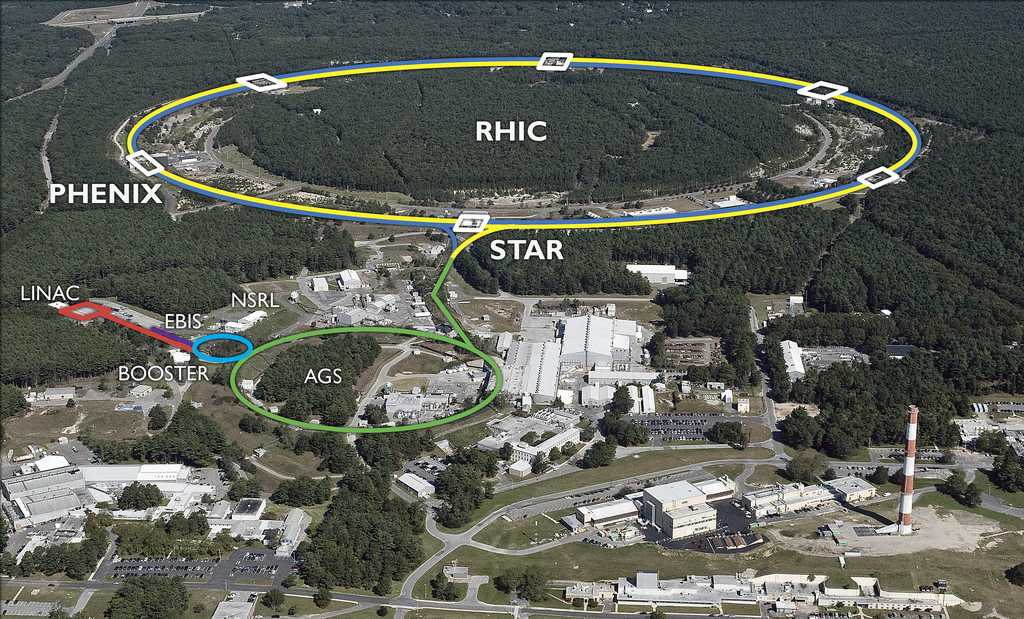
\includegraphics[width=0.6\textwidth]{Figures/RHIC-aerial-HR.jpg}
    \rule{35em}{0.5pt}
  \caption[An Aerial view of BNL]{An Aerial view of BNL with RHIC and the AGS outlined and the locations of PHENIX and STAR mapped}
  \label{fig:Aerial RHIC}
\end{figure}
\indent Based at Brookhaven National Lab (BNL) on the east end of Long Island, New York, the Relativistic Heavy Ion Collider (RHIC) is a particle accelerator and storage ring that is used to study the properties of nuclear matter, specifically the properties, formation of, and phase transition of nuclear matter into a novel state called the Quark Gluon Plasma (QGP).  RHIC accelerates nuclei which are stripped of their electrons (heavy ions) to almost the speed of light and collides them together with enough energy to raise the system's temperature to that which is required to create the QGP. 

\section{From Start to Finish}
\begin{figure}[htbp]
  \centering
    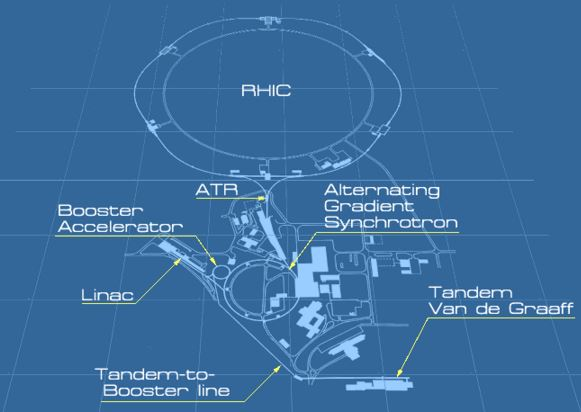
\includegraphics[width=0.8\textwidth]{Figures/RHICdiagram.JPG}
    \rule{35em}{0.5pt}
  \caption[Illustration of all the accelerators used to boost ions to relativistic speeds at RHIC]{Illustration of all the accelerators used to boost ions to relativistic speeds at RHIC}
  \label{fig:run8config}
\end{figure}
The speeds achieved at RHIC is the result of many smaller accelerators working in concert in order to boost the ions' speed faster and faster \citep{RHICaccel}.  Ions begin their journey at a compact source and heavy ion accelerator called the Electron Beam Ion Source (EBIS) (located by the Linear Accelerator (LINAC) in the diagram). From there they are transferred to the a circular accelerator called the Booster Synchrotron which utilizes long-wavelength radio frequency electromagnetic waves allowing the ions to "surf" on their downward slope. The ions are then fed into the Alternating Gradient Synchrotron (AGS). No slouch in and of itself, the AGS was once the proverbial end-of-the-line where experiments took place and were studied and is responsible for three Nobel Prizes itself: the discovery of the muon neutrino in 1962, the discovery of charge-parity violation in 1963, and the joint discovery of the J/$\Psi$ in 1976. The AGS uses the magnetic field gradients of 240 magnets, alternating them in order to boost the ions to 99.7$\%$ the speed of light after which it is transferred to the AGS-to-RHIC transfer line (AtR). The AtR is like a train switch yard wherein bunches of ions are fed into the RHIC rings. Bunches of ions are sent through either clockwise in one ring or counterclockwise in the other using a switching magnet.

RHIC is comprised of two concentric rings which are 3.8 kilometers in circumference.  These rings use 1,740 helium cooled superconducting magnets to hold beams of these heavy ions which circulate in opposite directions within the two rings.  Along the circumference of RHIC there are six points where the counter-circulating beams can be steered to collide (Interaction Regions or IR). Of these six IR, four have been used to house different detectors: the smaller, now defunct PHOBOS and BRAHMS experiments, and the larger still operational PHENIX and STAR experiments.  

RHIC is an incredibly flexible machine capable of colliding various species of nuclei from protons to Uranium \citep{EBISupgrade} at a wide range of energies.  Heavy ions such as Au can be accelerated as low as 3.85 $GeV/c^{2}$ and as high as 100 $GeV/c^{2}$ \citep{RHIClum} with a combined center of mass energy of 200 $GeV/c^{2}$.  When accelerating protons, RHIC is able to achieve up to 250 $GeV/u$ since the mass/charge ratio is smaller and is able to do so with polarized beams. It is also able to do this asymmetrically, that is to say, with two different species of nuclei, one in each ring.  The system studied in this thesis is one such asymmetric system wherein a deuteron is collided with a gold ion with a center of mass energy of 200 $GeV/c^{2}$ (this system is referred to shorthand as "d+Au").

\section{The PHENIX Detector}

\indent The analysis described in this thesis was made using the PHENIX detector which stands for: Pioneering High Energy Nuclear Interaction eXperiment. PHENIX is the largest of the experiments at RHIC and was designed specifically to study the QGP.  

\begin{figure}[htbp]
  \centering
    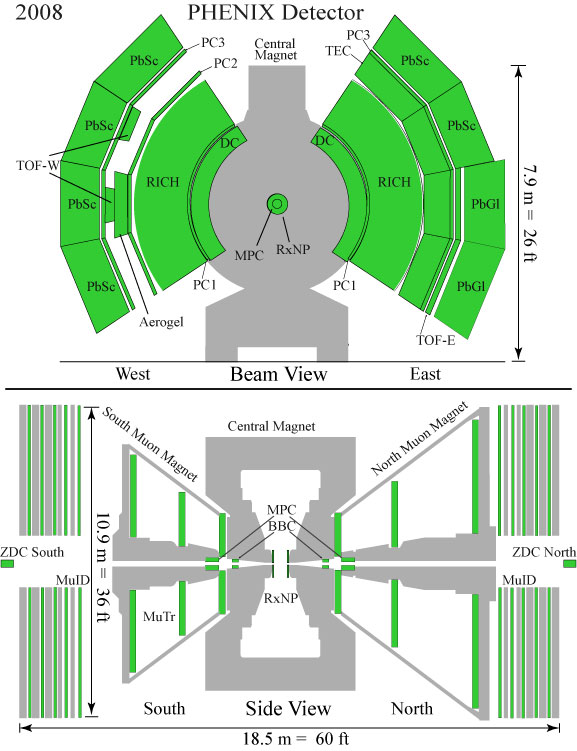
\includegraphics[width=0.8\textwidth]{Figures/Phenix_2008.jpg}
    \rule{35em}{0.5pt}
  \caption[PHENIX Detector Configuration for RHIC Run 8 (2008)]{The configuration of the PHENIX detector for Run 8 (2008)}
  \label{fig:run8config}
\end{figure}
%----------------------------------------------------------------------------------------
It consists of a collection of various detectors used to measure kinematic variables like track position, curvature, momentum, charge, time of flight. The muon arms are used for studying physics phenomena at forward rapidity ($\eta$ = $|1.1-2.4|$)\citep{rapidityref} but the system of detectors used for this analysis are contained in the Central Arm.  

\subsection{Central Arm}
Covering a rapidity range of $\eta$ = $<|0.375|$, the central arm consists of an east and a west arm that cover the azimuth $90^{\circ}$ each \citep{EMCfocus} and is shown on the upper image labeled "Beam View" on figure \ref{fig:run8config}. Particle trajectories are tracked using the Drift Chamber (DC) and the Pad Chambers (PC 1,2, and 3). In principle the DC is similar to a wire chamber; When a charged particle travels through the gas in the DC the gas atoms are ionized and these ions and electrons are accelerated to anode wires which collect this ionization and sends a signal proportional to the ionization effect of the traveling particle. The DC is filled with a gas that is selected to have a uniform drift velocity close to the anode wires, i.e. a gas such that the traveling ions and electrons in the ionized gas have a linear relation in position and time such that $x(t) = v_{drift} * t$ within the active region \citep{DCfocus}. In doing so and when combined with high accuracy timing caluculation we are able to achieve a more accurate position and trajectory of outgoing particles. The DC is the first detector that these outgoing particles passes through and is used in conjunction with other detectors in order to accurately determine track trajectory through all of the detectors in the central arm.
The Pad Chambers are three individual layers of pixel detectors. These pixels are arranged in 9 pixel clusters called "pads" that are readout by a single channel \citep{PCfocus}. The PC and DC have the same azimuthal coverage as the rest of the central arm and are located at increasing concentric distances from the collision vertex, the DC being the inner most detector, followed immediately by PC1.  PC2 only exists in the west arm however PC3 exists in both arms. This configuration is used to accurately determine particle track trajectories in order to match with other detector data such as calorimetry, time of flight, and Cherenkov counters.

\subsubsection{TOF: Time Of Flight Detectors}

In addition to the track matching detectors this analysis utilizes the Time of Flight (TOF) detectors which are high accuracy timing detectors that measure the time it takes for charged particles traveling through the central arm to go from the event vertex to the detector\citep{TOFfocus}. There are two TOF detectors in PHENIX, one on the east DC arm and one on the west arm. Located 5 meters away from the collision vertex and in the lower two sectors of the east arm, the TOF East (TOFE) is a scintillation detector with a timing resolution of $\Delta t_{res} \sim 80 ps$. It covers $\Delta\phi = \pi / 4$ and $\eta < |0.35|$. 

\begin{figure}[htbp]
  \centering
    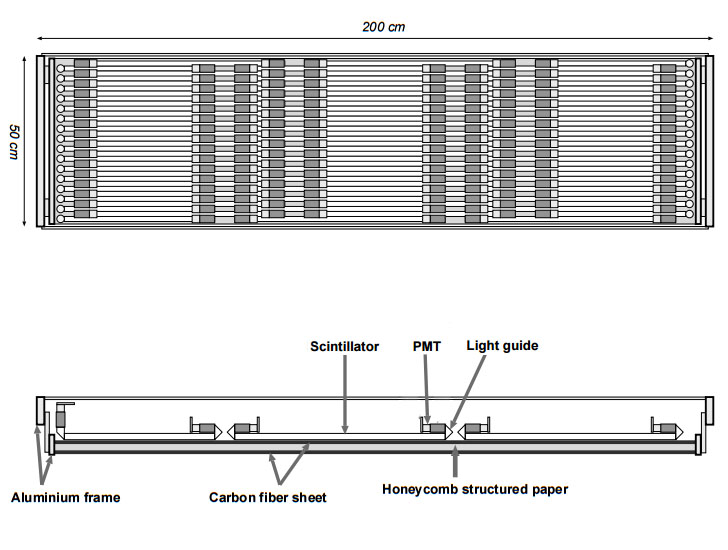
\includegraphics[width=0.8\textwidth]{Figures/TOFEschematic.jpg}
    \rule{35em}{0.5pt}
  \caption[A schematic of the slat layout in the TOFE]{A schematic of the slat layout in the TOFE}
  \label{fig:TOFEschematic}
\end{figure}

Scintillators are a special type of material that fluoresces when it absorbs radiation. The TOFE is comprised of 1000 "slats" of plastic scintillation material with two photomultiplier tubes (PMT) on either end of the slats which amplify the fluorescing photons caused by charged particles that pass through the scintillators. Since we know the length of the slat and the speed of light in the scintillation material we can easily calculate both the time when the particle first hit the slat ($T_{0}$) and the position where the particle hit the slat ($y$).

\begin{equation}
T_{0} = \frac{(T_{1}+T_{2})-L/v}{2} , \, \, y = \frac{T_{1}-T_{2}}{2} v
\end{equation}

Where $T_1$ and $T_{2}$ are the times measured by PMTs 1 and 2 respectively, $L$ is the length of the slat, and $v$ is the speed of light in the scintillator.

\begin{figure}[htbp]
  \centering
    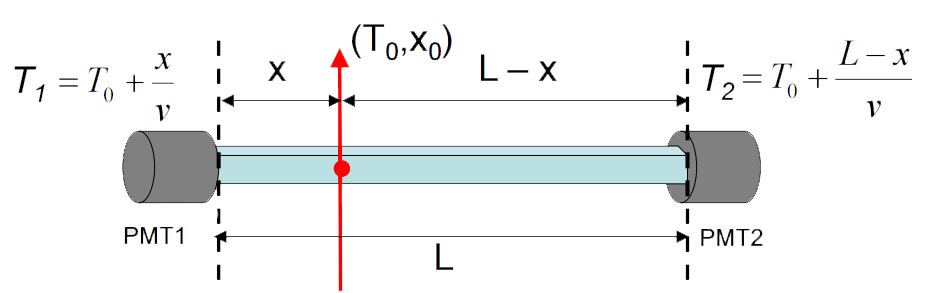
\includegraphics[width=0.8\textwidth]{Figures/TOFEcartoon.jpg}
    \rule{35em}{0.5pt}
  \caption[An illustration of a single slat in the TOFE]{An illustration of a single slat in the TOFE}
  \label{fig:TOFEcartoon}
\end{figure}

In the west arm, the TOF West (TOFW) is a 1024 channel Multi-gap Resistive Plate Chamber (MRPC) detector with a timing resolution of $\Delta t_{res} < 100 ps$, located 4.85 m from the collision vertex and also covering $\Delta\phi = \pi / 4$ and $\eta < |0.35|$. The MRPC works on the same principle as a basic Resistive Plate Chamber which is comprised of two high resistivity plastic (bakelite) plates separated by a volume of gas. On one resistive plate is a sheet of conducting material which is used to maintain a constant electric field across the gas gap. The other resistive plate has an array of conducting readout strips. When a charged particle travels through the gas it causes an electron avalanche similar to what happens in a drift chamber. This electron avalanche is accelerated under the influence of an externally applied electric field toward one of the readout strips resulting in a "hit" signal which is then amplified by electronics. 

\begin{figure}[h]
  \centering
    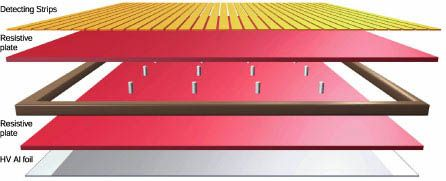
\includegraphics[width=0.8\textwidth]{Figures/RPClayers.jpg}
    \rule{35em}{0.5pt}
  \caption[Diagram of a basic RPC]{Diagram of a basic RPC \citep{CMSRPC}}
  \label{fig:RPCbasic}
\end{figure}

A MRPC is a version of an RPC with alternating layers of the  resistive material and gas gaps sandwiched together with the high voltage surface and readout strips on the outermost sides of the device \citep{Akindinov:2000rq}. The resistive plates inside the sandwich are electrically isolated and are transparent to the fast signals of incoming particles. Initially the externally applied electric field induces charges on the surfaces of the resistive plates causing each of the small gas gaps to be held at the same potential, and since each incoming particle ionizes the gas and deposits the same amount of one charge on one side of the plate and the opposite charge on the other, the potential in each individual gap is held constant. This means that the total signal the strips see is the \textit{sum} of all of the electrical activity in each of small gaps. By using this configuration a greater precision is allowed than conventional RPC designs and lends itself well to high precision timing detectors.

\begin{figure}[ht!]
  \centering
    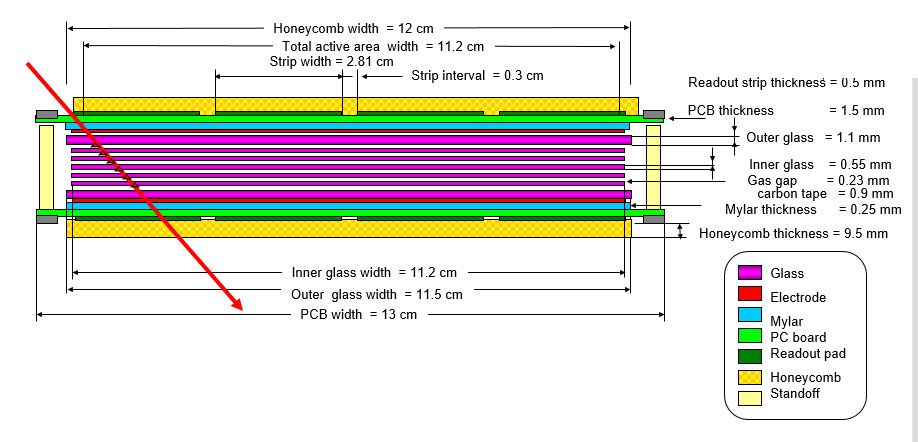
\includegraphics[width=0.8\textwidth]{Figures/MRPC_TOFW.jpg}
    \rule{35em}{0.5pt}
  \caption[Cross sectional diagram of the MRPCs used in the TOFW]{Cross sectional diagram of the MRPCs used in the TOFW}
  \label{fig:MRPCTOFW}
\end{figure}

\subsubsection{ACC: Aerogel Cherenkov Counter}
As track momentum increases the signal width of the particle masses increases. The high resolution capabilities of the TOF detectors only allows them to be able to separate $\pi^{\pm}$, $k^{\pm}$, and $p$ / $\bar{p}$ signals up to certain transverse momentum $p_{T}$ thresholds. The distinct masses of the particles of interest do provide an additional method of separating particle signals since if you were to give two particles of different mass the same momentum they would have distinct velocities. This is the principle with which a Cherenkov detector works. Cherenkov radiation is light that is emitted in a material when a charged particle travels through it with a velocity faster than the speed of light in that medium. This medium called a Cherenkov radiator can be carefully selected such that its intrinsic speed of light is such that lighter particles with higher velocities cause Cherenkov radiation but heavier particles which travel slower given the same momentum will not. Using this, a Cherenkov detector acts as a logic detector categorizing tracks as those that either "fire" or "veto", that is to say tracks that radiate versus tracks that don't. In the case of separating $\pi^{\pm}$ mesons from $k^{\pm}$ mesons for $p_{T}$ tracks where their mass signals overlap so strongly that they cannot be uncorrelated, the radiator was chosen such that the pions will fire the detector and the kaons will not. Pions and kaons are indistinguishable for $p_{T} > 2.8$ GeV/c, so the radiator chosen to separate the signals is a silica aerogel ($n \approx 1.011$).

\begin{figure}[htbp!]
  \centering
    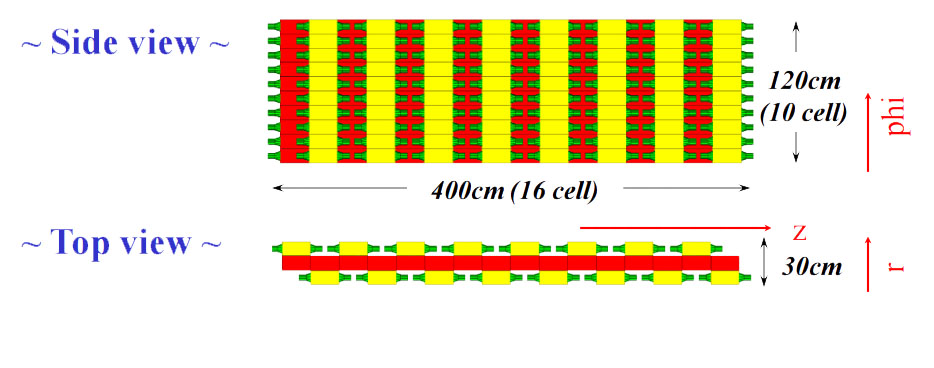
\includegraphics[width=0.8\textwidth]{Figures/ACCschematic.jpg}
    \rule{35em}{0.5pt}
  \caption[A schematic of the Aerogel Cherenkov Counter]{A schematic of the Aerogel Cherenkov Counter}
  \label{fig:ACCschematic}
\end{figure}

The Aerogel Cherenkov Counter (ACC) is comprised of 160 tiles of silica aerogel. Each tile is affixed to an integration cube which allows for radiated cherenkov photons to reflect internally until they hit a PMT. Each integration cube is filled with air and is covered on all exposed sides by a goretex reflector except for the "front" facing aerogel tile side and the two cutouts where the PMTs attach. There are two PMTs located opposite from each other for each cube. To account for the space taken by PMTs on the ends of the tiles the ACC is two sided and the tiles are oriented such that the opposite side tile occupies the gap where PMTs would be situated.  There are 10 rows of 8 tiles on each side for a total of 160 tiles.

\begin{figure}[htbp!]
  \centering
    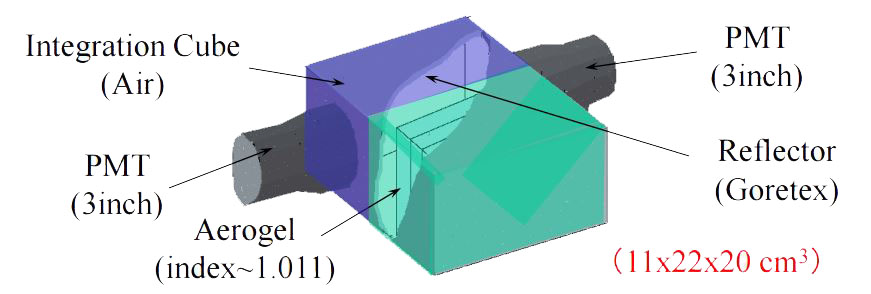
\includegraphics[width=0.8\textwidth]{Figures/aerogelchannel.JPG}
    \rule{35em}{0.5pt}
  \caption[A schematic of one tile in the ACC]{A schematic of one tile in the ACC}
  \label{fig:accchannel}
\end{figure}

The ACC is located in the west arm covering the half of the azimuthal coverage that the TOFW covers and with the same rapidity coverage. When used in conjunction with the TOFW it can provide pion/kaon separation for $p_{T} < 4$ GeV/c and can discriminate protons for $p_{T} < 7$ GeV/c.  The total capabilities of the combination of the TOFW + ACC is shown in the following chart.

\begin{figure}[h!]
  \centering
    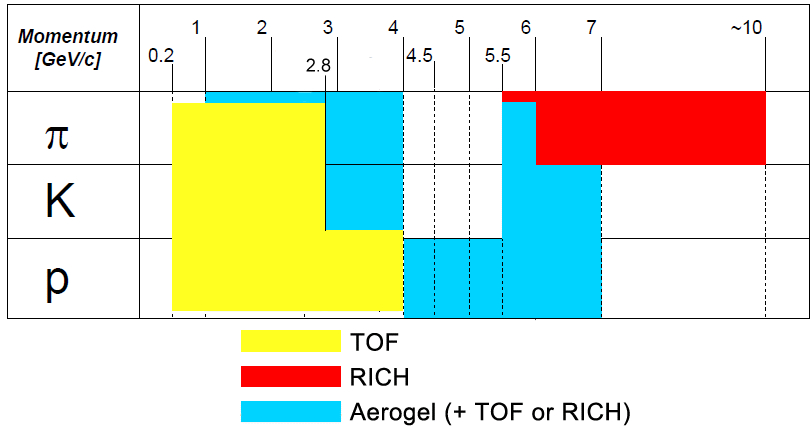
\includegraphics[width=0.8\textwidth]{Figures/accrange.jpg}
    \rule{35em}{0.5pt}
  \caption[Chart of Particle Identification capabilities over a range of transverse momentum]{Chart of Particle Identification capabilities over a range of transverse momentum}
  \label{fig:PIDrange}
\end{figure}


\subsection{Forward Detectors}
Though the bulk of this analysis is dependent on the central arm detectors, many components such as the start of the event timer, the event vertex, centrality, and event reaction plane are dependent on a handful of forward detectors which I will briefly discuss here.

\subsubsection{BBC: Beam-Beam Counter}
Of the forward detectors, the \textit{Beam-Beam Counter} (BBC) is probably the most important because of its ability to measure the various global event parameters. There are two BBCs, one on the north side and one on the south side of PHENIX both equidistant from the center of the interaction region (IR). The constituent detector elements are made of quartz Cherenkov radiators attached to meshed dynode PMTs housed in hexagonal encasement. These elements are arranged in a toroidal shape in order to allow the ion beams to pass through the center while still getting full $2\pi$ azimuthal coverage. The BBCs cover 3.1$\leq \Delta \eta \leq<$4 in pseudorapidity.
\begin{figure}
\centering
\begin{subfigure}[b]{0.4\textwidth}
    \centering
    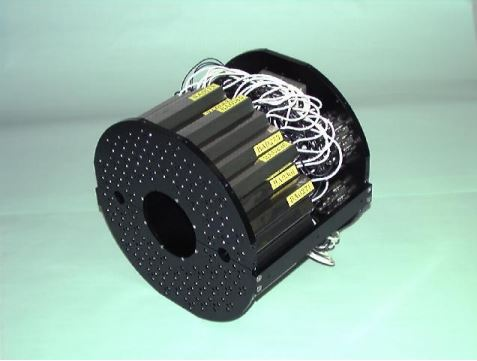
\includegraphics[width=\textwidth]{Figures/bbcrender.JPG}
    \caption{An illustration of a BBC}
    \label{fig:ppiratiocentvsperiph}
\end{subfigure}
\begin{subfigure}[b]{0.4\textwidth}
    \centering
    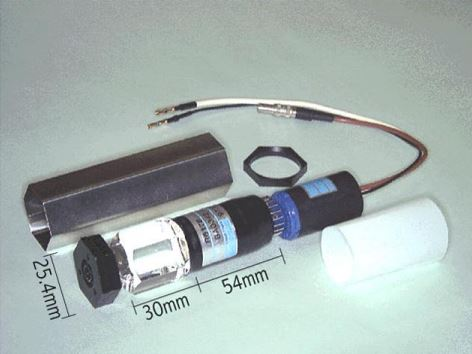
\includegraphics[width=\textwidth]{Figures/bbcsinglechannel.JPG}
    \caption{A single element of the BBC}
    \label{fig:Rcpcentvsperiph}
\end{subfigure}
\caption[The Beam Beam Counter]{The Beam Beam Counter}
\label{fig:baryonenhancementAA}
\end{figure}

\subsubsection{ZDC/SMD: Zero Degree Calorimeter and Shower Max Detectors}
Crucial to the determination of event centrality is the ability to count the number of spectator particles. Since neutrons are have no charge we can place a calorimeter at high rapidity behind an IR dipole magnet which we can use to "sweep" away charged particles like proton spectators and other charged track noise. The \textit{Zero Degree Calorimeter}\citep{ZDCfocus} is comprised of a ribbon of acrylic fiber optic strands sandwiched between two tungsten plates. The tungsten plates act as a dense absorber for the neutrons to hit and shower into resulting in detectable photon yield in the fiber optic ribbon. Sandwiched between modules of the ZDC is a hodoscope called the \textit{Shower Max Detector} (SMD). The SMD is comprised of 21 0.5 cm x 0.5 cm scintillators and is used to measure the centroid of the shower in cartesian coordinates since the ZDC only measures energy\citep{phenixzdc}. The ZDC is used in conjunction with the BBC in order to determine centrality. Since more peripheral collisions mean more spectators and therefore more neutrons to hit the ZDC, the higher the energy measured by the ZDC the more peripheral the event (see fig \ref{fig:zdcvsbbc}\citep{Ghosh2001}).

\begin{figure}[h!]
  \centering
    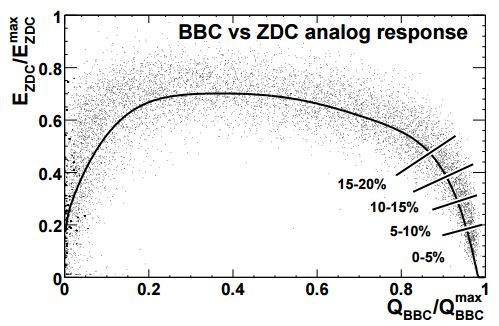
\includegraphics[width=0.5\textwidth]{prevplots/bbczdcanaresponse.JPG}
    \rule{35em}{0.5pt}
  \caption[Centrality bins as determined by ZDC energy versus BBC charge sum]{Centrality bins as determined by ZDC energy versus BBC charge sum\citep{Ghosh2001}}
  \label{fig:zdcvsbbc}
\end{figure}

\subsubsection{MPC: Muon Piston Calorimeter}
The \textit{Muon Piston Calorimeter} (MPC) was a needed upgrade to PHENIX that provided calorimetry at very high rapidity\citep{kleinjanthesis}. It was installed in two parts: first in the south in 2005, then in the north in 2006 and was commisioned to reconstruct $\pi^{0}$ and $\eta$ mesons for various forward physics analyses. Nestled in a gap in the piston of the Muon Magnet Arms, it provides full azimuthal coverage at $3.1 \leq  | \eta | \leq 3.7$ ($3.9$ in the north) and is comprised of 196 (220 in the north) Lead Tungstate $PbWO_4$ crystal scintillator towers attached to avalanche photodiodes with preamplifiers to measure the electromagnetic shower photons. For this analysis, the MPC is used as a another measurement point for determining the reaction plane resolution correction. 

\begin{figure}[h!]
  \centering
    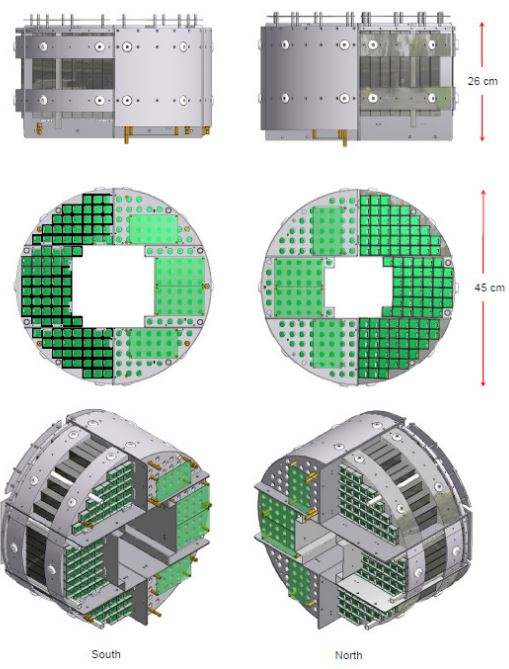
\includegraphics[width=0.5\textwidth]{Figures/mpcschematic.JPG}
    \rule{35em}{0.5pt}
  \caption[Schematic of the MPC]{Schematic of the MPC}
  \label{fig:mpcschematic}
\end{figure}

\subsubsection{RXNP: Reaction Plane Detector}

Each arm has full coverage of Electromagnetic Calorimeters (EMCal) in eight sectors, four sectors each. Six of the sectors (all four of the west arm and the top two in the east arm) are made of channels comprised of alternating layers of lead and scintillator (PbSc). The lower two sectors in the east arm are comprised of a uniform lead glass Cherenkov radiator (PbGl). 

\pagebreak
\pagebreak
